\documentclass[twoside,10pt]{article}
\usepackage{shlists}
\usepackage[spanish]{babel}
\usepackage[applemac]{inputenc}
\usepackage[T1]{fontenc}

\usepackage{multicol}
\usepackage{picinpar}

\usepackage{url}
\newcommand{\surl}[1]{{\small\url{#1}}}

\newcounter{vol}
\newcounter{num}
\newcounter{anyo}
\setcounter{vol}{8}
\setcounter{num}{3}
\setcounter{anyo}{2014}
\newcommand{\mes}{Septiembre}
\usepackage{revisionNLcol}


\title{\ \\ Docencia 2.0\\ \large Juan Juli\'an Merelo, Fernando 
Tricas}
\author{\LARGE Control de versiones y el ecosistema a su alrededor}

\date{}

\AutTit{Docencia 2.0}

\begin{document}
\addtocounter{page}{2}

\maketitle
\vspace*{-2ex}

\begin{multicols}{2}

Los proyectos en ingenier\'ia, en general, se desarrollan por equipos. Y los
equipos necesitan herramientas para controlar qui\'en hace qu\'e, incorporar
cambios a trav\'es de un proceso establecido y poder, en caso necesario,
ver la evoluci\'on del dise\~no a trav\'es de las versiones del mismo.
En el caso del desarrollo de sistemas inform\'aticos tambi\'en es
posible, y
necesario en algunos casos, volver a alg\'un punto anterior del trabajo,
corregir alg�n error introducido en una versi�n anterior o explorar caminos alternativos. 

En ingenier\'ia inform\'atica los sistemas que incorporan esas
caracter�sticas se denominan sistemas de 
gesti\'on de c�digo fuente o de control de versiones. Son programas que
gestionan el acceso por parte de un equipo al c\'odigo fuente, en
archivos de texto guardados en diferentes directorios, de un
proyecto. Bien desde la l\'inea de \'ordenes o desde un interfaz gr\'afico,
permiten  {\em comprometer} un fichero o un grupo de ficheros que han
cambiado, crear diferentes {\em ramas} de desarrollo y fusionarlas con
una serie de \'ordenes simples. 
El trabajo concurrente sobre un mismo proyecto provocar\'a
necesariamente la necesidad de coordinarse. Pero de manera casi
inevitable se producir\'an conflictos: 
cuando dos miembros del equipo han modificado la misma l\'inea, hay que
determinar si se trata de un error, un desajuste respecto a las
especificaciones o, simplemente, diferentes formas de abordar un problema; el
sistema de control de versiones marcar\'a sobre el texto las l\'ineas en
las que se ha producido el conflicto, mostrando las dos versiones, y nos
obligar\'a a solucionarlo eligiendo, eliminando o modificando la l\'inea o
l\'ineas que hayan causado el conflicto.

Hoy en d\'ia cualquier empresa con un m\'inimo departamento TIC usa, o
deber\'ia usar, un sistema de control de versiones; entre todos los
existentes uno de los que m\'as atracci\'on ha ganado es
{\tt git}, dise\~nado inicialmente por Linus Torvalds con su experiencia en la
gestion del desarrollo del kernel de Linux pero hoy en d\'ia convertido en el
est�ndar \textsl{de facto}; hoy en d�a lo mantiene y desarrolla Junio Hamano. 
Permite el desarrollo con equipos distribuidos, de manera no necesariamente
lineal e incluye un sistema de publicacion web de los repositorios, entre
otras caracter\'\i sticas interesantes.

Entender el funcionamiento de git como principal sistema de control de
versiones en la actualidad y 
sus patrones de trabajo es fundamental en la carrera de inform\'atica, tan
fundamental como trabajar con un lenguaje de programaci\'on de {\em
scripting} o
entender el idioma ingl\'es. Y lo es
hasta tal punto que debe ser una habilidad transversal como lo es usar
Internet. Esto es, no  algo incluido de una asignatura como
Ingenier\'ia del Software, sino una parte integral del curr\'iculum de todas y
cada una de las asignaturas de una carrera de Inform\'atica. 
Tampoco ser\'a raro que el inform\'atico termine encontr\'andose con estas
herramientas cuando explore el c\'odigo de otros, en cualquier caso.

Porque el aprendizaje del ingeniero debe prepararle, a trav\'es de la
pr\'actica, para su trabajo y la mejor forma de hacerlo es usando las
mismas herramientas para que su uso se interiorice y se desarrollen
estrategias propias para el mismo. Porque 
\noindent\rule{86mm}{1pt}

%--------------------------
\vspace{1ex} {\small{\begin{window}[0,r,
\includegraphics[width = 27
mm]{JJM.jpg},] \noindent\emph{JJ Merelo} es catedr\'{a}tico de Universidad
en el \'area de Arquitectura y Tecnolog\'{\i}a de Computadores, y
actualmente director de la Oficina de Software Libre de la UGR.
Mantiene un blog desde el a\~no 2002, y lo ha utilizado en clase desde
el a\~no 2004; tambi\'en wikis y, ultimamente, agregadores y otras
herramientas TIC. \'{U}ltimamente le ha dado por el \textsl{flipped
learning}, de lo que se informar\'{a} debidamente en esta columna.
\end{window}}}

\medskip

{\small{\begin{window}[0,r,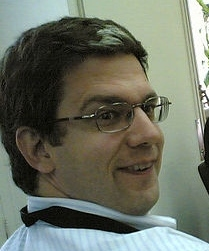
\includegraphics[width = 27 mm]{FTricas1.jpg},]
		\noindent  \emph{Fernando Tricas Garc\'{\i}a} es profesor
		titular de Lenguajes y Sistemas Inform\'aticos del Departamento
		de Inform\'atica e Ingenier\'{\i}a de Sistemas de la Universidad de
		Zaragoza.  Empez\'o a estudiar la blogosfera casi cuando a\'un no
		exist\'{\i}a (all\'a por el a\~no 2002) y a tratar de integrarla en los
		cursos y tareas docentes un poco despu\'es.  Ha impartido
		numerosas charlas relacionadas con el tema de la Web 2.0.
		Es actualmente Director de su departamento.  
		\end{window}}}
%-------------------------------------------------

\noindent no cabe duda de
que usar git puede ayudar en todas y cada una de las asignaturas para
desarrollar trabajos en grupo y elaborar documentos de la misma
forma. Pero adem\'as, al ser por omisi\'on una herramienta de trabajo en
grupo, permite desarrollar estrategias de organizaci\'on de este tipo de
trabajo que son tambi\'en \'utiles para el empleo posterior.

Por \'ultimo, pero no por ello menos importante, trabajar con
repositorios de git p\'ublicos como GitHub hace que el alumno desarrolle
un portafolio de trabajos realizados que ser\'an su mejor carta de
presentaci\'on para obtener empleo y 
 presentar su trabajo a la comunidad
de desarrolladores. De hecho, muchas empresas de recursos humanos
hacen \textsl{mining} de repositorios git para encontrar a empleados que
correspondan a un 
perfil y nivel de habilidad requerido por una empresa. 

Todo ello sin dejar de lado las caracter\'isticas sociales de estos sitios, que
nos pueden permitir conocer proyectos interesantes, desarrolladores de los que
aprender y, en definitiva, tejer esa red de aprendizaje que nos puede dar
soporte en el futuro para nuestros propios proyectos.

Aunque el uso no es mayoritario, git (y otros sistemas de control de
versiones) tambi\'en pueden utilizarse para todo tipo de archivos de
texto, por ejemplo, documentaci\'on o escritura colaborativa de un trabajo.
Incluso para gestionar un blog (con Jekyll, por ejemplo). Los fuentes (en \LaTeX) de estas
columnas est\'an alojados en GitHub y uno de nosotros (J. J. Merelo,
junto con Pablo Hinojosa) public\'o en Amazon un libro sobre git que tambi\'en
est\'a alojado  en GitHub: \surl{https://github.com/oslugr/curso-git}. 

Tambi\'en hemos estado experimentando (tanto en repositorios p\'ublicos
como privados) con la publicaci\'on de datos de experimentos, por la
simplicidad a la hora de gestionar grandes cantidades de informaci\'on,
tenerlas disponibles en la web, compartirlas... 

En resumen, git es el verdadero sistema operativo de los equipos de trabajo
en inform\'atica. Y como tal debe ocupar una
posici\'on privilegiada dentro de la ense\~nanza de la misma.




\bigskip

\noindent\emph{Todas las columnas de la serie Docencia 2.0
pueden descargarse en formato LaTeX desde
\surl{https://github.com/ReVision-Docencia-20/Columnas}}

\noindent\rule{90mm}{1pt}

{\small \noindent\copyright 2015 JJ. Merelo, F. Tricas. Este art\'{\i}culo es de acceso libre distribuido bajo los t\'erminos
de la Licencia Creative Commons de Atribuci\'on, que permite copiar,
distribuir y comunicar p\'ublicamente la obra en cualquier medio, s\'olido
o electr\'onico, siempre que se acrediten a los autores y fuentes
originales}

\end{multicols}
\end{document}
	








\end{multicols}
\end{document}
 
